\scanpage{68}
\[
K(x)\longrightarrow\coprod_y K(y)
\]
\diagram{$\left\{\vcenter{\hbox{\begin{tikzcd}[ampersand replacement=\&,row sep=small]
x\arrow[d]\\x'\arrow[d]\\x''
\end{tikzcd}}}\right.$}
\diagram{\begin{tikzcd}[ampersand replacement=\&,column sep=large]
K(x)\arrow[r]\&\displaystyle\coprod_{x'\,\text{précède}\,x}K(x')\arrow[d]\\
\&\displaystyle\coprod_{x''\,\text{\unsure{biprécède}}\,x}K(x'')
\end{tikzcd}}
\margin{$K(x)\unsure{\longrightarrow|-}\displaystyle\prod_{x'\,\text{\unsure{pré}}}$}
\[
\underbrace{K(x)\longrightarrow\coprod_{\substack{x'\\\text{\unsure{les intermédiaires}}\\\text{entre }x\text{ et }x''}}K(x')\longrightarrow K(x'')}_{\text{nul}}
\]
\[
\deleted{\operatorname{Hom}(K(x),K(y))}
\]
\[
\begin{aligned}
\operatorname{Hom}(K,K)&=\prod_x\operatorname{Hom}(K(x),K)\\
&=\prod_x\prod_y^{\text{\unsure{restreint}}}\underbrace{\operatorname{Hom}(K(x),K(y))}_{H(x,y)}
\end{aligned}
\]
$H(x,x)$ \unsure{un anneau}
\[
H(x\qquad K\rightsquigarrow I
\]
\figure{\begin{tikzpicture}
\draw[->] (0,0)--(4,.3);\foreach \x in {0,.8,1.6,2.4,3.2}{\draw (\x,-.05+.075*\x)--(\x,.08+.075*\x);}
\draw[->,dashed] (0,.1)..controls(1.4,1.4)and(3.6,1)..(4.1,.3);
\end{tikzpicture}}
\[
\operatorname{Hom}(K,
\]
\diagram{\begin{tikzcd}[ampersand replacement=\&,row sep=small,column sep=large]
\unsure{q|\varphi}\mid\arrow[r,dash]\&{}\arrow[rr,dash,very thick]\&{}\&K(y')\arrow[d]\\
\&K(x)\arrow[u]\arrow[urr,shift left]\arrow[urr,shift right]\arrow[rr,dash]\arrow[dr]\&{}\&K(y)\\
\&{}\&K(x')\arrow[ur]\&{}
\end{tikzcd}}
\figure{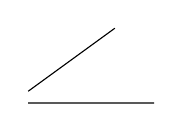
\begin{tikzpicture}\draw (0,0)--(1.1,.8) (0,-.15)--(1.6,-.15);\end{tikzpicture}}
\[
\unsure{q|\mathfrak q}\supset\unsure{p|\mathfrak p}\qquad K(p)\longrightarrow I
\]
\figure{
\begin{tikzpicture}\draw (0,0)--(.5,.8) (.08,0)--(.58,.8);\end{tikzpicture}}
\[
\operatorname{Hom}(K,D(A))
\]
\inserted{\unsure{un cas particulier}}
\diagram{\begin{tikzcd}[ampersand replacement=\&,column sep=large,row sep=small]
\&\&*\arrow[d,"d'_{\unsure{g|q}}"]\\
\bullet\arrow[urr,Rightarrow]\arrow[rr,Rightarrow]\arrow[dr,"d"']\&\&\deleted{\unsure{\theta}}\arrow[dr,"d'"]\\
\&\bullet\arrow[rr]\&\&\bullet
\end{tikzcd}}
\diagram{\begin{tikzcd}[ampersand replacement=\&,column sep=small,row sep=small]
\&{}\arrow[dr,"d"]\&\&\&\\
\&\&{}\arrow[dr,"d"]\&\&\\
\bullet\arrow[uur,"3"]\arrow[urr,"2"]\arrow[rrr,"1"]\arrow[dr,"d"']\&\&\&\bullet\arrow[dr,"d"]\&\\
\&{}\arrow[uur,"3"]\arrow[urr,"2"]\arrow[rrr,"1"']\arrow[dr,"d"']\&\&\&{}\\
\&\&{}\arrow[uur,"3"]\arrow[urr,"2"']\arrow[dr,"d"']\&\&\\
\&\&\&\bullet\arrow[uur,"3"']\&
\end{tikzcd}}
\figure{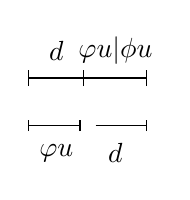
\begin{tikzpicture}
\draw[thick] (0,.6)--(1.5,.6); \foreach \x in {0,.7,1.5}{\draw (\x,.5)--(\x,.7);}
\node at (.35,.95) {$d$};\node at (1.1,.95) {$\unsure{\varphi u|\phi u}$};
\draw (0,0)--(.65,0) (.85,0)--(1.5,0);\draw (0,-.07)--(0,.07) (.65,-.07)--(.65,.07) (1.5,-.07)--(1.5,.07);
\node at (.35,-.35) {$\unsure{\varphi u}$};\node at (1.1,-.35) {$d$};
\end{tikzpicture}}
\figure{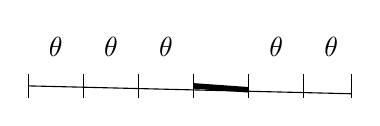
\begin{tikzpicture}
\draw (0,0)--(4.1,-.1);\foreach \x in {0,.7,1.4,2.1,2.8,3.5,4.1}{\draw (\x,-.15)--(\x,.15);}
\draw[line width=2pt] (2.1,0)--(2.8,-.05);
\foreach \x in {.35,1.05,1.75,3.15,3.85}{\node at (\x,.5) {$\theta$};}
\end{tikzpicture}}
\figure{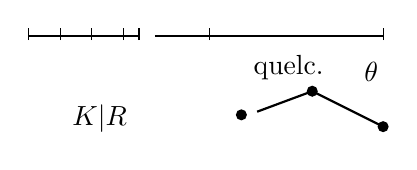
\begin{tikzpicture}
\draw[thick] (0,1)--(1.4,1) (1.6,1)--(4.5,1);\foreach \x in {0,.4,.8,1.2,1.4,2.3,4.5}{\draw (\x,.95)--(\x,1.1);}
\node at (.9,-.05) {$\unsure{\mathscr K|\mathscr R}$};
\fill (2.7,0) circle(2pt) (3.6,.3) circle(2pt) (4.5,-.15) circle(2pt);
\draw[thick] (2.9,.04)--(3.6,.3)--(4.5,-.15);
\node at (3.3,.6) {\unsure{quelc.}};\node at (4.35,.55) {$\theta$};
\end{tikzpicture}}
% archive sheet number: 67
